\chapter{Практическая часть}
\label{ch:practice}

\section{Установка стека LAMP}

Для установки полного стека LAMP используется утилита \texttt{tasksel}.
Отвечает на вопросы установщика в неинтерактивном режиме переменная
\texttt{DEBIAN\_FRONTEND=noninteractive}:
\begin{lstlisting}
apt-get install -y tasksel
DEBIAN_FRONTEND=noninteractive tasksel install lamp-server
\end{lstlisting}

Дополнительно устанавливаются PHP-расширения, необходимые WordPress:
\begin{lstlisting}
apt-get install -y php-curl php-gd php-mbstring php-xml \
    php-xmlrpc php-soap php-intl php-zip
\end{lstlisting}

% --- Скриншот: статус Apache2 ---
\begin{figure}[h]
  \centering
  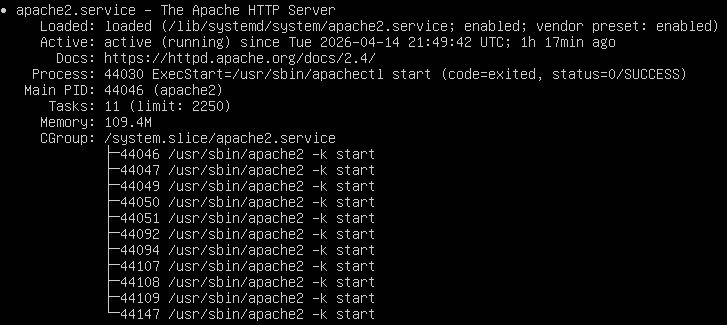
\includegraphics{img/04_apache2_status}
  \caption{Сервис Apache2 успешно запущен после установки LAMP}
  \label{fig:apache_status}
\end{figure}

\section{Настройка Apache2}

Для предотвращения предупреждения \texttt{AH00558} в \texttt{apache2.conf}
добавляется директива \texttt{ServerName}:
\begin{lstlisting}
echo "ServerName localhost" >> /etc/apache2/apache2.conf
\end{lstlisting}

Настраиваются права на директорию сайта:
\begin{lstlisting}
chown -R www-data:www-data /var/www
chmod -R 755 /var/www
systemctl restart apache2
\end{lstlisting}

Создаётся файл Virtual Host для WordPress:
\begin{lstlisting}
<VirtualHost *:80>
    ServerName 192.168.29.6
    ServerAlias wordpress.yazikov.iks531.local
    DocumentRoot /var/www/html
    <Directory /var/www/html>
        AllowOverride All
        Require all granted
    </Directory>
</VirtualHost>
\end{lstlisting}

Активируется сайт и модуль rewrite:
\begin{lstlisting}
a2ensite wordpress.conf
a2dissite 000-default.conf
a2enmod rewrite
systemctl restart apache2
\end{lstlisting}

% --- Скриншот: файл Virtual Host ---
\begin{figure}[h]
  \centering
  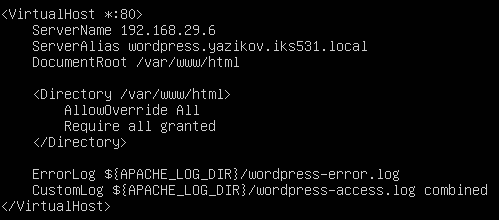
\includegraphics{img/05_vhost_conf}
  \caption{Конфигурация Virtual Host Apache для WordPress}
  \label{fig:vhost}
\end{figure}

\section{Настройка MariaDB и создание базы данных}

После установки LAMP запускается MariaDB и создаётся база данных
для WordPress:
\begin{lstlisting}
systemctl enable mariadb
systemctl start mariadb
\end{lstlisting}

Устанавливается пароль root и создаётся база данных с пользователем:
\begin{lstlisting}
mysqladmin -u root password 'DB_PASSWORD'
mysql -u root -p'DB_PASSWORD' <<SQL
CREATE DATABASE IF NOT EXISTS wordpress
    CHARACTER SET utf8 COLLATE utf8_bin;
CREATE USER IF NOT EXISTS 'author'@'localhost'
    IDENTIFIED BY 'DB_PASSWORD';
GRANT ALL PRIVILEGES ON wordpress.*
    TO 'author'@'localhost';
FLUSH PRIVILEGES;
SQL
\end{lstlisting}

\section{Установка и настройка WordPress}

Скачивается архив русской версии WordPress и распаковывается:
\begin{lstlisting}
cd /tmp
wget https://ru.wordpress.org/latest-ruRU.tar.gz \
    -O wordpress.tar.gz
tar xzvf wordpress.tar.gz
\end{lstlisting}

Настраивается \texttt{wp-config.php} --- заменяются параметры
подключения к базе данных:
\begin{lstlisting}
cp wp-config-sample.php wp-config.php
sed -i "s/database_name_here/wordpress/" wp-config.php
sed -i "s/username_here/author/"        wp-config.php
sed -i "s/password_here/DB_PASSWORD/"  wp-config.php
\end{lstlisting}

Файлы WordPress разворачиваются в корень сайта Apache:
\begin{lstlisting}
rm -f /var/www/html/index.html
rsync -aq /tmp/wordpress/ /var/www/html/
chown -R www-data:www-data /var/www/html
chmod -R 755 /var/www/html
\end{lstlisting}

% --- Скриншот: файлы WordPress в /var/www/html ---
\begin{figure}[h]
  \centering
  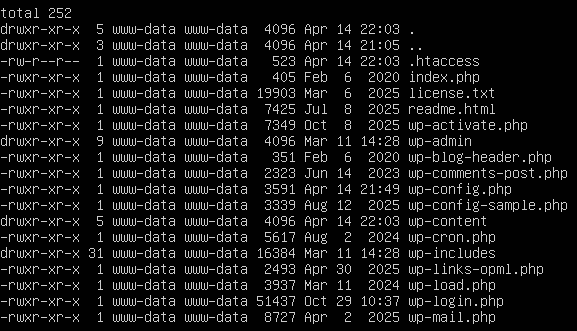
\includegraphics{img/07_wp_files}
  \caption{Файлы WordPress развёрнуты в /var/www/html}
  \label{fig:wp_files}
\end{figure}

\section{Интерактивная установка WordPress через браузер}

После завершения скрипта на ВМ \texttt{desktop1} открывается
браузер Firefox и выполняется переход по адресу
\texttt{http://\cfgWpIP/}. Открывается мастер установки WordPress.

Заполняются поля мастера:
\begin{itemize}
  \item Название сайта: \texttt{\cfgDomain};
  \item Имя пользователя: \texttt{admin};
  \item Пароль: надёжный пароль;
  \item Email: \texttt{admin@\cfgDomain}.
\end{itemize}

После нажатия кнопки \textit{«Установить WordPress»} система
создаёт таблицы в базе данных и перенаправляет на страницу входа.

% --- Скриншот: успешная установка ---
\begin{figure}[h]
  \centering
  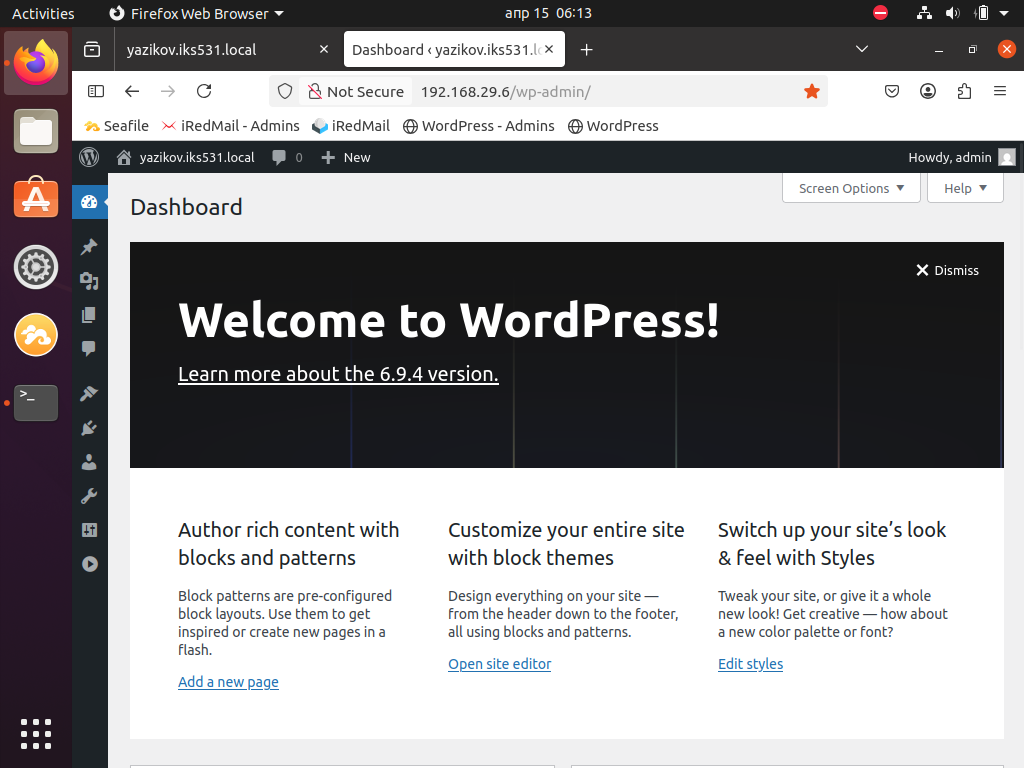
\includegraphics{img/09_wp_install_success}
  \caption{Успешное завершение установки WordPress}
  \label{fig:wp_success}
\end{figure}

\section{Проверка работы сайта}

После входа в панель администратора \texttt{http://\cfgWpIP/wp-admin}
создаётся тестовая запись: меню \textit{Записи} → \textit{Добавить
новую} → заполняется заголовок и текст → публикуется.

Проверяется отображение записи на главной странице сайта
\texttt{http://\cfgWpIP/}.

% --- Скриншот: тестовая запись на главной странице ---
\begin{figure}[h]
  \centering
  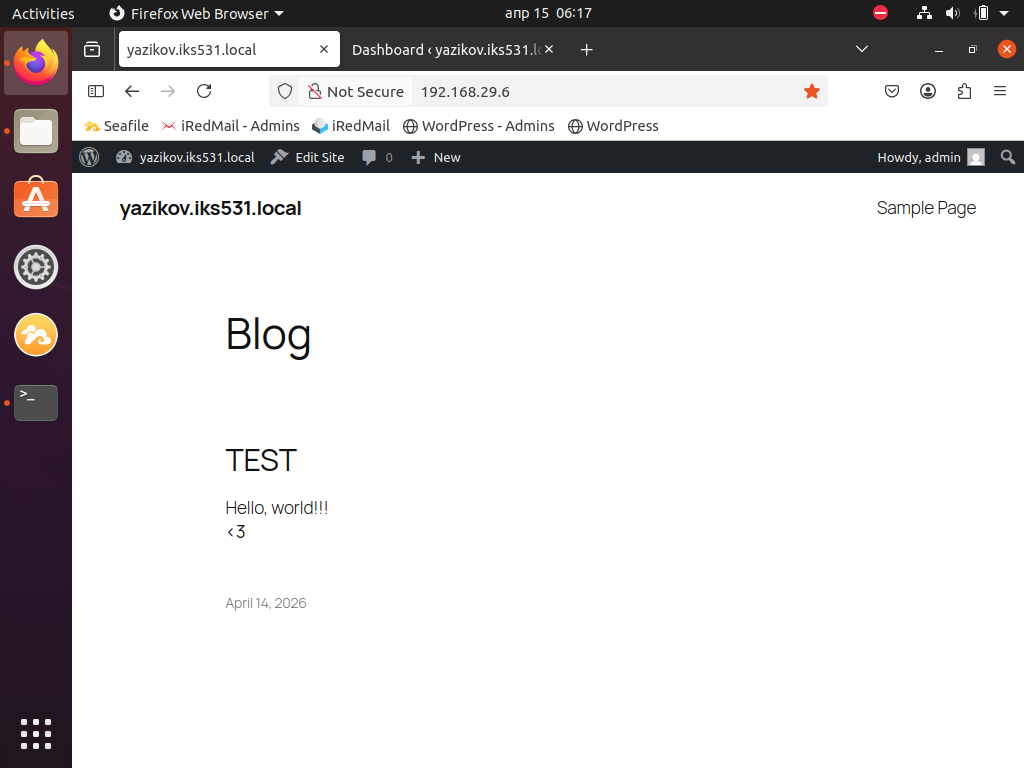
\includegraphics{img/11_wp_post_published}
  \caption{Тестовая запись опубликована и отображается на главной странице}
  \label{fig:wp_post}
\end{figure}

\section{Результаты проверки}

Проверка состояния сервисов и доступности выполняется скриптом
\texttt{wordpress\_lab8\_post.sh}:
\begin{lstlisting}
sudo bash lab8/wordpress_lab8_post.sh
\end{lstlisting}

Ожидаемый результат:
\begin{itemize}
  \item \texttt{apache2} и \texttt{mariadb} --- статус \texttt{active (running)};
  \item порты 80 и 3306 --- слушаются;
  \item HTTP-запрос к \texttt{http://\cfgWpIP/} возвращает код 200 или 302;
  \item \texttt{wp-login.php} доступен;
  \item база данных \texttt{wordpress} доступна пользователю \texttt{author}.
\end{itemize}

% --- Скриншот: результат wordpress_lab8_post.sh ---
\begin{figure}[h]
  \centering
  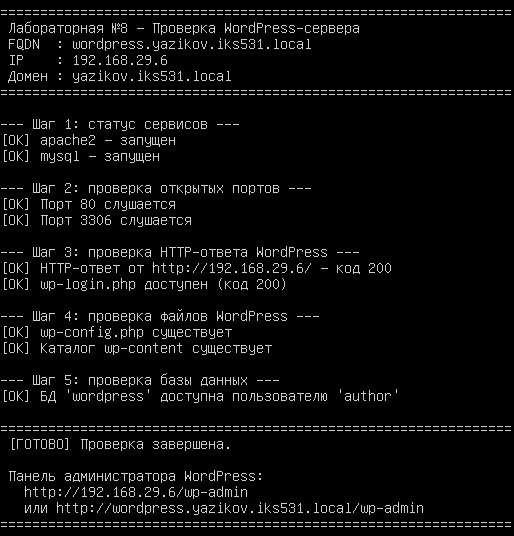
\includegraphics{img/12_post_check}
  \caption{Результат проверочного скрипта wordpress\_lab8\_post.sh}
  \label{fig:post_check}
\end{figure}

\endinput
